\let\lesson\undefined
\newcommand{\lesson}{\phantomlesson{Bài 22: Động lực học của chuyển động tròn. Lực hướng tâm}}
\chapter[Động lực học của chuyển động tròn. Lực hướng tâm]{Động lực học của chuyển động tròn. Lực hướng tâm}
\setcounter{section}{0}
\section{Lý thuyết}
\subsection{Lực hướng tâm}
\begin{center}
	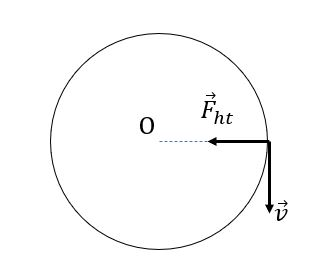
\includegraphics[scale=0.6]{../figs/VN10-PH-16-L-013-1-V2-04.JPG}
\end{center}
\subsubsection{Định nghĩa}
Lực (hay hợp lực của các lực) tác dụng vào một vật chuyển động tròn đều và gây ra cho vật gia tốc hướng tâm gọi là lực hướng tâm.
\subsubsection{Biểu thức}

\begin{equation*}
	F_{\text{ht}} = m \cdot a_{\text{ht}} = m\dfrac{v^2}{r},
\end{equation*}
trong đó:
\begin{itemize}
	\item $m$ là khối lượng của vật (kg), 
	\item $v$ là tốc độ dài của vật (m/s),
	\item $r$ là bán kính quỹ đạo (m),
	\item $F_{\text{ht}}$ là lực hướng tâm (N).
\end{itemize}
\section{Mục tiêu bài học - Ví dụ minh họa}
\begin{dang}{Ghi nhớ công thức tính lực hướng tâm, đặc điểm của lực hướng tâm}
	\viduii{1}{Chọn phát biểu sai về lực hướng tâm:
		\begin{mcq}
			\item Vệ tinh nhân tạo chuyển động tròn đều quanh Trái Đất do lực hấp dẫn đóng vai trò lực hướng tâm.
			\item Xe chuyển động vào một đoạn đường cong (khúc cua), lực đóng vai trò hướng tâm luôn là lực ma sát.
			\item Xe chuyển động đều trên đỉnh một cầu võng, hợp lực của trọng lực và phản lực vuông góc đóng vai trò lực hướng tâm.
			\item Vật nằm yên đối với mặt bàn nằm ngang đang quay đều quanh trục thẳng đứng thì lực ma sát nghỉ đóng vai trò lực hướng tâm.
		\end{mcq}
	}
	{	\begin{center}
			\textbf{Hướng dẫn giải}
		\end{center}
		
		Nếu mặt đường nghiêng vào trong tâm quỹ đạo cong thì hợp lực của phản lực $N$ và trọng lực $P$ khi xe qua đoạn đường cong cũng đóng góp vào lực hướng tâm, không phải chỉ có lực ma sát.
		
		\textbf{Đáp án: B}.
	}
	\viduii{1}{Một vật có khối lượng $m$ đang chuyển động tròn đều trên một quỹ đạo bán kính $r$ với tốc độ góc $\omega$. Lực hướng tâm tác dụng vào vật được xác định bởi
		\begin{mcq}(2)
			\item $F_\text{ht} = m\omega^2 r.$
			\item $F_\text{ht} = \dfrac{mr}{\omega}.$
			\item $F_\text{ht} = \omega^2 r.$
			\item $F_\text{ht} = m\omega^2 .$
		\end{mcq}
	}
	{	\begin{center}
			\textbf{Hướng dẫn giải}
		\end{center}
		
		Lực hay hợp lực của các lực tác dụng lên một vật chuyển động tròn đều và gây ra cho vật gia tốc hướng tâm gọi là lực hướng tâm.
		
		$$F_\text{ht} = ma_\text{ht} = m\dfrac{v^2}{r} = m\omega^2 r.$$
		
		\textbf{Đáp án: A}.
	}
	
\end{dang}
\begin{dang}{Xác định lực hướng tâm trong trường hợp vật chuyển động qua cung tròn}
	\viduii{3}{Lấy $g=\SI{10}{m/s^2}$. Tính áp lực của ô tô 4 tấn đi qua điểm giữa cầu với tốc độ $\SI{72}{km/h}$ trong các trường hợp sau:
		\begin{enumerate}[label=\alph*)]
			\item Cầu phẳng.
			\item Cầu cong lồi bán kính $\SI{100}{m}$.
			\item Cầu cong lõm bán kính $\SI{100}{m}$.
		\end{enumerate}
	}
	{	\begin{center}
			\textbf{Hướng dẫn giải}
		\end{center}
		
		\begin{itemize}
			\item Trọng lực $\vec P$ của ô tô và phản lực $\vec N$ của mặt cầu tác dụng lên ô tô đóng vai trò lực hướng tâm 
			\begin{equation*}
				\vec{F}_{\text{ht}} = \vec{P} +\vec{N}.
			\end{equation*}
			\item Áp dụng định luật III Newton, áp lực $\vec Q$ do ô tô tác dụng lên cầu $\vec Q=\vec N$.
		\end{itemize}
	\begin{enumerate}[label=\alph*)]
		\item Cầu phẳng
		\begin{center}
			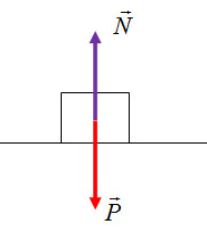
\includegraphics[scale=0.5]{../figs/VN10-PH-16-L-013-1-V2-01.JPG}
		\end{center}
		\begin{equation*}
		 N=P=mg=\left(\SI{4E3}{\kilogram}\right)\cdot\left(\SI{10}{\meter/\second^2}\right)=\SI{40000}{\newton}.
		\end{equation*}
	\item Cầu cong lồi
	\begin{center}
		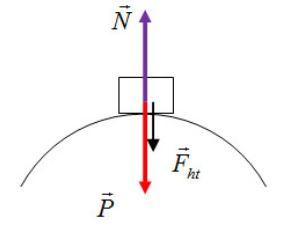
\includegraphics[scale=0.5]{../figs/VN10-PH-16-L-013-1-V2-02.JPG}
	\end{center}
	\begin{equation*}
		F_{\text{ht}} =P-N\Rightarrow  N=P-F_{\text{ht}} =mg-m\dfrac{v^2}{r}=\left(\SI{4E3}{\kilogram}\right)\cdot\left(\SI{10}{\meter/\second^2}\right)-\left(\SI{4E3}{\kilogram}\right)\cdot\dfrac{\left(\SI{20}{\meter/\second}\right)^2}{\SI{100}{\meter}}=\SI{24000}{\newton}.
	\end{equation*}
\item Cầu cong lõm
\begin{center}
	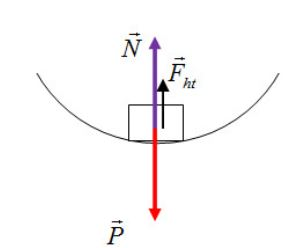
\includegraphics[scale=0.5]{../figs/VN10-PH-16-L-013-1-V2-03.JPG}
\end{center}
\begin{equation*}
	F_{\text{ht}} =N-P\Rightarrow  N=P+F_{\text{ht}} =mg+m\dfrac{v^2}{r}=\left(\SI{4E3}{\kilogram}\right)\cdot\left(\SI{10}{\meter/\second^2}\right)+\left(\SI{4E3}{\kilogram}\right)\cdot\dfrac{\left(\SI{20}{\meter/\second}\right)^2}{\SI{100}{\meter}}=\SI{56000}{\newton}.
\end{equation*}
	\end{enumerate}
	}
	\viduii{3}{Một xe có khối lượng $m$ chuyển động trên đường cua tròn có bán kính $r = \SI{100}{m}$ với tốc độ không đổi $\SI{72}{km/h}$. Lấy $g = \SI{10}{m/s^2}$. Hệ số ma sát giữa lốp xe và mặt đường ít nhất bằng bao nhiêu để xe không trượt?
	}
	{	\begin{center}
			\textbf{Hướng dẫn giải}
		\end{center}
		
		Đổi đơn vị $\SI{72}{km/h}=\SI{20}{m/s}$.
		
		Xe chuyển động tròn đều nên lực ma sát nghỉ đóng vai trò là lực hướng tâm.
		
		Để xe không trượt trên đường thì:
		
		$$F_\text{ht} = F_\text{msn}\le F_\text{msn max} \Leftrightarrow m\dfrac{v^2}{r} \leq \mu mg.$$
		
		$$\Rightarrow \mu \geq \dfrac{v^2}{gr} =\dfrac{\left(\SI{20}{\meter/\second}\right)^2}{\left(\SI{10}{\meter/\second^2}\right)\cdot\left(\SI{100}{\meter}\right)}= \SI{0,4}{}\Rightarrow \mu_\text{min} =\SI{0,4}{}$$
	}
	%\end{dang}
	%\begin{dang}{Xác định lực hướng tâm \\là hợp lực của trọng lực và phản lực }
	\viduii{3}{Một xô nước coi như chất điểm có khối lượng tổng cộng là $\SI{2}{kg}$ được buộc vào sợi dây dài $\SI{0,8}{m}$. Người ta quay dây với tốc độ góc 45 vòng/phút trong mặt phẳng đứng. Tính lực căng của dây khi xô đi qua điểm cao nhất và điểm thấp nhất của quỹ đạo.
	}
	{	\begin{center}
			\textbf{Hướng dẫn giải}
		\end{center}
	\begin{minipage}[l]{0.65\textwidth}
		Trong quá trình xô nước chuyển động tròn, hợp lực của lực căng dây $\vec T$ và trọng lực  $\vec P$ của vật đóng vai trò là lực hướng tâm:
		\begin{equation}
			\label{eq:32.1}
			\vec P+\vec T=m\vec a_\text{ht}
		\end{equation}
		Chiếu phương trình (\ref{eq:32.1}) lên phương bán kính, chiều dương hướng vào tâm quỹ đạo.
		\begin{itemize}
			\item Lực căng dây ở vị trí cao nhất:
			\begin{equation*}
				P+T =F_{\text{ht}} \Rightarrow T = m(\omega^2R -g)=\SI{15,9}{N}.
			\end{equation*}
			\item Lực căng dây ở vị trí thấp nhất: 
			\begin{equation*}
				-P+T =F_{\text{ht}} \Rightarrow T = m(\omega^2R +g)=\SI{55,1}{N}.
			\end{equation*}
		\end{itemize}
	\end{minipage}
\begin{minipage}[l]{0.3\textwidth}
	\begin{center}
		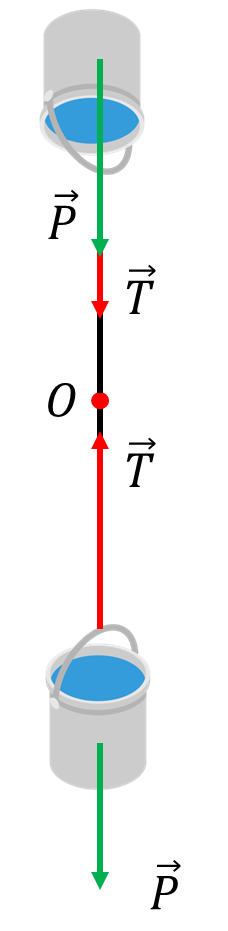
\includegraphics[width=0.3\linewidth]{../figs/VN10-2023-PH-TP032-1}
	\end{center}
\end{minipage}
		
	}
	\viduii{4}{Một máy bay thực hiện vòng nhào lộn bán kính $\SI{400}{m}$ trong mặt phẳng đứng với tốc độ $\SI{540}{km/h}$. Lấy $g = \SI{10}{m/s^2}$.
		\begin{enumerate}[label=\alph*)]
			\item Tính lực do người lái có khối lượng $\SI{60}{kg}$ nén lên ghế ngồi ở điểm cao nhất và thấp nhất của vòng nhào lộn.
			\item Tốc độ máy bay phải bằng bao nhiêu để người lái không nén lên ghế?
		\end{enumerate}
	}
	{	\begin{center}
			\textbf{Hướng dẫn giải}
		\end{center}
	\begin{minipage}[l]{0.65\textwidth}
		Theo định luật III Newton, lực do người nén lên ghế ngồi $\vec Q=-\vec N$.\\
		Trong quá trình máy bay thực hiện nhào lộn, phản lực  $\vec N$ do ghế tác dụng lên người và trọng lực  $\vec P$ của người đóng vai trò là lực hướng tâm:
		\begin{equation}
			\label{eq:32.2}
			\vec P+\vec N=m\vec a_\text{ht}
		\end{equation}
		Chiếu phương trình (\ref{eq:32.2}) lên phương bán kính, chiều dương hướng vào tâm quỹ đạo.
	\end{minipage}
	\begin{minipage}[l]{0.3\textwidth}
		\begin{center}
			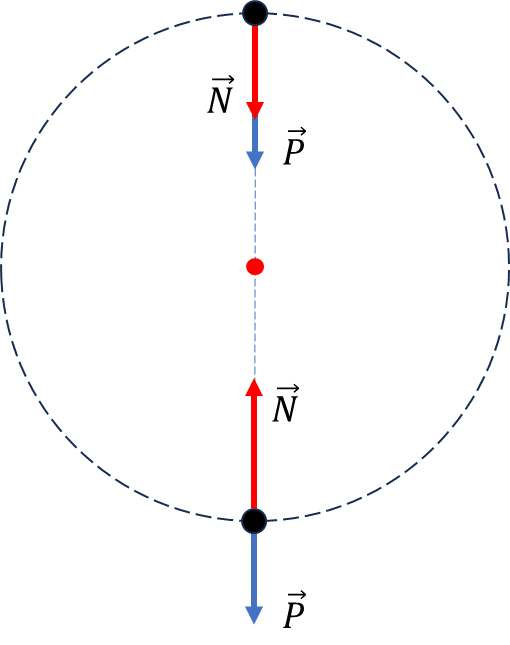
\includegraphics[width=0.7\linewidth]{../figs/VN10-2023-PH-TP032-2}
		\end{center}
	\end{minipage}
		\begin{enumerate}[label=\alph*)]
			\item 
			\begin{itemize}
				\item Tại điểm thấp nhất áp lực của người lái nén lên ghế ngồi là
				\begin{equation*}
					N=P+F_{\text{ht}} = mg +\dfrac{mv^2}{R} =\left(\SI{60}{\kilogram}\right)\cdot\left(\SI{10}{\meter/\second^2}\right)+\dfrac{\left(\SI{60}{\kilogram}\right)\cdot\left(\SI{150}{\meter/\second}\right)^2}{\SI{400}{\meter}}=\SI{3975}{N}.
				\end{equation*} 
				\item Tại điểm cao nhất áp lực của người lái nén lên ghế ngồi là
				\begin{equation*}
					N=-P+F_{\text{ht}} = -mg +\dfrac{mv^2}{R} =-\left(\SI{60}{\kilogram}\right)\cdot\left(\SI{10}{\meter/\second^2}\right)+\dfrac{\left(\SI{60}{\kilogram}\right)\cdot\left(\SI{150}{\meter/\second}\right)^2}{\SI{400}{\meter}}= \SI{2775}{N}.
				\end{equation*} 
			\end{itemize}
			\item Để người lái không nén lên ghế thì phản lực do ghế tác dụng lên người tại điểm cao nhất $N=0$, suy ra 
			\begin{equation*}
				F_{\text{ht}}=P \Leftrightarrow mg = \dfrac{mv^2}{R} \Rightarrow v =\sqrt {gR} =\sqrt{\left(\SI{10}{\meter/\second^2}\right)\cdot\left(\SI{400}{\meter}\right)}\approx\SI{63.25}{\meter/\second}.
			\end{equation*}
		\end{enumerate}
	
	}
	\viduii{4}{Diễn viên xiếc đi xe đạp trên vòng xiếc bán kính $\SI{6,4}{m}$. Lấy $g = \SI{10}{m/s^2}$. Để đi qua điểm cao nhất mà không rơi thì người đó phải đi với tốc độ tối thiểu bằng bao nhiêu?
	}
	{	\begin{center}
			\textbf{Hướng dẫn giải}
		\end{center}
		\begin{center}
			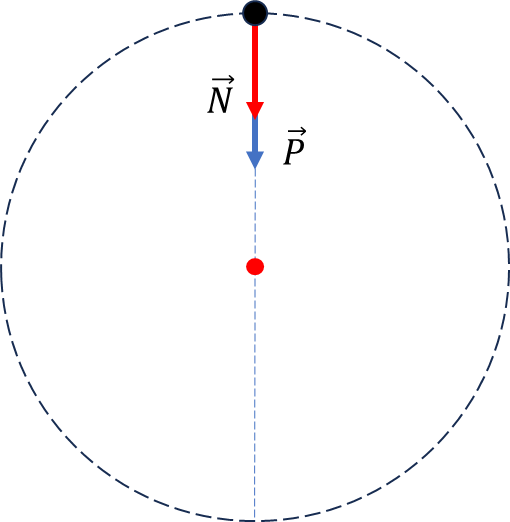
\includegraphics[width=0.3\linewidth]{../figs/VN10-2023-PH-TP032-3}
		\end{center}
		Tại điểm cao nhất của vòng xiếc có các lực tác dụng lên xe là trọng lực $\vec P$ và phản lực  $\vec N$ của vòng xiếc.	
		\begin{equation}
			\label{eq:32.3}
			\vec P+\vec N=m\vec a_\text{ht}
		\end{equation}
	Chiếu phương trình (\ref{eq:32.2}) lên phương bán kính, chiều dương hướng vào tâm quỹ đạo:
		$$P + N = m \dfrac{v^2}{R} \Rightarrow N  =  m \dfrac{v^2}{R} - P =m \dfrac{v^2}{R}-mg .$$
		
		Muốn không bị rơi khỏi vòng xiếc thì vẫn còn lực ép lên vòng xiếc. Khi đó $N \geq 0 $, suy ra
		
		$$ m \dfrac{v^2}{R}-mg \geq 0 \Rightarrow v \geq \sqrt{gR} =\sqrt{\left(\SI{10}{\meter/\second^2}\right)\cdot\left(\SI{6.4}{\meter}\right)}=\SI{8}{\meter/\second} \Rightarrow v_\text{min} = \SI{8}{m/s}.$$
		
		
	}
	
\end{dang}